\documentclass[../../General.tex]{subfiles}
\begin{document}

\section{Definición de la problemática}

La implementación de instrumentación en plantas fotovoltaicas se enfrenta a un desafío logístico y técnico considerable: la heterogeneidad de las condiciones climáticas dentro de una misma instalación \citep{Salinas2025}. A medida que los proyectos a gran escala se asientan sobre terrenos con topografías complejas, como las vistas en la Figura \ref{fig:PlantaPeru}, se generan microclimas que provocan variaciones espaciales significativas. Por ejemplo, las diferencias de elevación alteran localmente los perfiles aerodinámicos del viento, mientras que las variaciones topográficas causan una distribución desigual de la radiación solar. Estudios en plantas de gran tamaño demuestran empíricamente que esta dispersión geográfica puede generar diferencias de hasta un 20\,\% en la irradiación diaria y fluctuaciones extremas superiores al 40\,\% a nivel horario, así como variaciones térmicas de 6 a 7 °C entre paneles separados dentro de una planta solar \citep{Garcia2014}. 




\begin{figure}[H]
	% Fuerza la alineación izquierda y quita los ":" después del número
	\captionsetup{justification=raggedright, singlelinecheck=false, labelsep=none}
	
	\caption[Imagen aérea de planta de energía solar en inmediaciones de la fábrica de cemento Yura, Arequipa.]{} 
	
	\textit{Imagen aérea de planta de energía solar en inmediaciones de la fábrica de cemento Yura, Arequipa.} \par\medskip
	
	\centering
	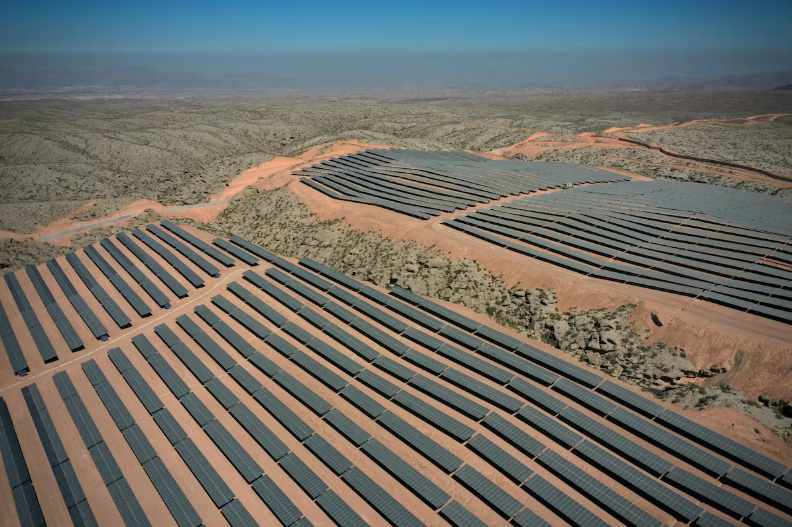
\includegraphics[width=0.6\textwidth]{Recursos/Imagenes/Otros/PlantaPeru.png} \par\medskip
	
	\raggedright
	\footnotesize \textit{Nota.} Fotografía adaptada sobre la noticia ``Yura y el poder del sol'' \citep{YuraPeru}.
	\label{fig:PlantaPeru}
\end{figure}


Para hacer frente a esta variabilidad y cumplir con los requisitos de monitorización de normativas internacionales, como la IEC 61724-1 \citep{IEC61724-1_2021}, las plantas recurren actualmente a la instalación de estaciones meteorológicas y redes de instrumentación fijas. En el contexto de un parque fotovoltaico, una estación meteorológica se concibe como un núcleo de monitorización centralizado mediante un adquisidor de datos, el cual integra una serie de instrumentos de alta precisión para caracterizar el recurso solar y el entorno climático \citep{Anatrac}. Típicamente, esta estación está equipada con piranómetros, sensores de temperatura ambiente, anemómetros y medidores de humedad relativa y presión atmosférica \citep{ProyectoEjecutivo2024}. Sin embargo, depender exclusivamente de puntos de medición estáticos presenta severas limitaciones. En la práctica, unos pocos sensores asumen un terreno plano y homogéneo, por lo que son físicamente incapaces de capturar con precisión la variabilidad climática real a lo largo de relieves montañosos y terrenos extensos \citep{Salinas2025}.

En consecuencia, el problema central se define como la ineficiencia de los métodos de instrumentación estáticos para caracterizar adecuadamente este mosaico de microclimas a lo largo de una planta fotovoltaica. Dado que los datos recopilados por la instrumentación fija no son verdaderamente representativos de las condiciones que experimentan los módulos en las distintas elevaciones del terreno, los operadores se enfrentan a una alta incertidumbre en la evaluación de los índices de rendimiento energético y a deficiencias importantes para la detección y localización oportuna de fallas operativas.

A esta falta de representatividad espacial se suma el enorme desafío financiero de intentar escalar o densificar la red de monitoreo instalando más estaciones fijas para cubrir el terreno. Adquirir y mantener múltiples estaciones meteorológicas de grado comercial representa un gasto logístico y económico notable, el cual puede llegar a constituir hasta el 1,6\,\% del presupuesto total de ejecución material de un proyecto fotovoltaico \citep{Burriana5MW}. Dado que resulta material y financieramente inviable instalar estos instrumentos fijos en cada zona del relieve, se evidencia la necesidad de transitar hacia métodos de inspección dinámicos y móviles que sean verdaderamente representativos de todo el entorno solar a un costo razonable.

\end{document}

